\section{Considerações Finais}

Feito todo esse processo, conectamos o ESP32 ao computador com o cabo USB. Com o atalho $Alt+Ctrl+U$, o processo para o envio do código é iniciado. Ao finalizar, o resultado já é visível e podemos manipular o eixo do potenciômetro para alterar a intensidade do LED vermelho e publicar os resultados diferentes no gráfico no ThingSpeak.

\begin{figure}[H]
    \centering
    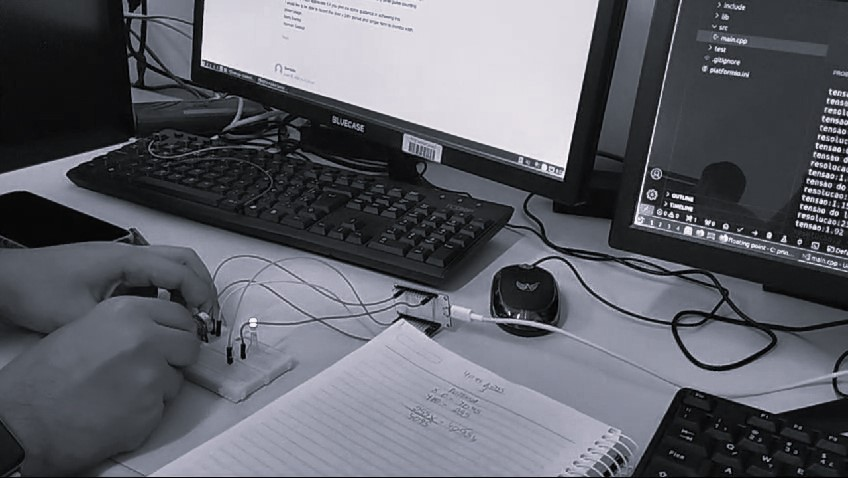
\includegraphics[width=0.5\linewidth]{img/resultado.jpg}
    \caption{Resultado final.}
    \label{fig:result}
\end{figure}

É possível conferir o resultado da prática por meio desse \href{https://youtu.be/2tGOsjk8wQs}{vídeo} no YouTube. O código completo está disponível nesse \href{https://github.com/fabricio-araujo94/microcontroladores/tree/main/potenciometro}{repositório} no GitHub.